%!TEX program=xelatex
%!TEX program=bibtex
%!TEX program=xelatex
%!TEX program=xelatex
% !Mode:: "TeX:UTF-8"
\documentclass[master,openany,twoside,a4paper,AutoFakeBold]{sudathesis}
\usepackage{tikz-dependency}
\usepackage{graphicx}
\usepackage{tikz}
\usepackage{tikz-qtree}
\usepackage{caption}
\usepackage{bbm}
\usepackage{letltxmacro}
\usepackage{mathtools}
\usepackage{pgfplots}
\usepackage{dashrule}
\usepackage[hang,flushmargin]{footmisc} % no indentation for footnotes
%\usepackage[SlantFont,BoldFont,CJKchecksingle,CJKnumber]{xeCJK}
%\setmainfont[BoldFont=SimHei ,ItalicFont=KaiTi_GB2312]{SimKai}
%\newcommand\fontnamekai{KaiTi_GB2312}

\usepackage{graphics}
\usepackage{pdfpages}

\newfontfamily\tgtermes{TeX Gyre Termes}
\makeatletter
  \begingroup
    \tgtermes
    \DeclareFontShape{\f@encoding}{\rmdefault}{m}{sc}{%
      <-> ssub * \f@family/m/sc}{}
    \DeclareFontShape{\f@encoding}{\rmdefault}{bx}{sc}{%
      <-> ssub * \f@family/bx/sc}{}
  \endgroup
\makeatother
\newcommand*\tcircle[1]{%
  \raisebox{.5pt}{\textcircled{\raisebox{-.9pt} {#1}}}
}

\begin{document}

% 论文相关信息
% !Mode:: "TeX:UTF-8"

% 学院中英文名,中文不需要“学院”二字
% 院系英文名可从以下导航页面进入各个学院的主页查看
% http://www.buaa.edu.cn/xyykc/index.htm
\school
{计算机科学与技术学院}{School of XXX}

% 专业中英文名
\major
{计算机科学与技术~~~}{XXXX Engineering}

% 方向中英文名
\direct
{自然语言处理~~}{XXXX Engineering}

% 论文中英文标题
\thesistitle
{这是中文标题}{ABCDEFG-test title}


% 作者中英文名
\thesisauthor
{张宇~~~~}{Yu Zhang}

% 导师中英文名
\teacher
{李正华}{Zhenghua Li}


% 班级
\class{XXXX}

% 学号
\studentID{20184227035}

% 单位代码
\unicode{10285}

% 论文时间,用于首页
\thesisdate{2021}{6}


\maketitle


\includepdf[page=-]{pdf-pages/独创性声明.pdf}

\includepdf[page=-]{pdf-pages/空白页.pdf}

\includepdf[page=-]{pdf-pages/授权声明.pdf}

\includepdf[page=-]{pdf-pages/空白页.pdf}

% 正文前页码是大写罗马字母
\pagenumbering{Roman}
% 前言页眉页脚样式 % 摘要
\pagestyle{cnfrontmatter}
% !Mode:: "TeX:UTF-8"

% 中英文摘要
\begin{cabstract}
	句法分析任务是句子理解的重要中间过程之一.
	其中,概率估计一直是句法分析领域的一个核心问题.
	然而,无论是神经网络方法还是深度学习时代以前的方法,采用基于全局概率模型的句法分析工作都非常少,主要的原因在于树形条件随机场(TreeCRF)推断的高复杂度.
	在本文中,我们提出将TreeCRF应用到依存句法和成分句法这两个主要的句法分析任务.
	为了解决TreeCRF的低效问题,关键的想法是批次化树结构的推断算法,并且用基于自动求导的反向传播代替Outside算法.
	目前句法模型被不断简化,采用局部损失目标是当前句法分析方法的一个趋势,我们则进一步在一阶TreeCRF的基础上采用了高阶拓展.
	高阶TreeCRF进一步增加了算法复杂度,为此,我们还提出利用基于平均场变分推断的近似推断算法代替精确推断的TreeCRF方法,从而增加了解析效率.
	
	\vskip 21bp
	{\heiti\zihao{-4} 关键词:}
	句法分析,
	依存句法分析,
	成分句法分析,
	树形条件随机场,
	变分推断
	
	\begin{flushright}
		作~~~~~~~~者:张~~~~宇
		
		指导老师:李正华
		
	\end{flushright}
\end{cabstract}




\pagestyle{enfrontmatter}
% !Mode:: "TeX:UTF-8"

\begin{eabstract}
	Syntactic parsing is one of the most important intermediate processes in sentence comprehension,
	and probability estimation has always been a core problem in the parsing field.
	However, in either deep learning (DL) era or pre-DL era, there exist very few works based on global probabilistic modeling, mainly due to the high complexity of tree-structure CRF (TreeCRF) inference.
	This thesis proposes to apply TreeCRF to both dependency parsing and constituency parsing.
	The key idea to solve the inefficiency issue is to batchify the inference algorithm for tree structures, and meanwhile avoid the complex Outside algorithm via back-propagation.
	Currently, parsing models are greatly simplified, and it's a trend to adopt local loss for syntactic parsing.
	In contrast, we propose a high-order extension to first-order models.
	While high-order modeling further increases the algorithm complexity, we also try to apply mean field variational inference (MFVI) as an alternative to exact inference of TreeCRF method, which greatly improves the parsing efficiency.

	\vskip 21bp
	{\bf\zihao{-4} Key words: }
	Syntactic Parsing,
	Dependency Parsing,
	Constituency Parsing,
	TreeCRF,
	Variational Inference
\end{eabstract}

\begin{flushright}
	Written by Yu Zhang
	
	Supervised by Zhenghua Li
\end{flushright}


% 目录不设置页眉和页码
\makeatletter
\let \asas \ps@plain
\let \ps@plain \ps@empty
\makeatother
\pagestyle{empty}

% 生成目录
\tableofcontents
\setcounter{secnumdepth}{4}

\makeatletter
\let \ps@plain \asas
\let\asas\relax
\makeatother
\clearpage  %目录3页以上,使用cleardoublepage

% 正文页码样式
\mainmatter
% 正文页眉页脚样式
\pagestyle{mainmatter}
% 正文页码是阿拉伯数字
\pagenumbering{arabic}

% % 正文

\chapter{绪论}

\section{研究背景和意义}
中文参考文献\cite{li-2013-chinese-dep}

英文参考\cite{krahenbuhl-etal-2011-efficient}
\chapter{第二章xx}

\chapter{第三章xx}
\chapter{第四章xx}
\chapter{总结与展望}

% % 参考文献,4或者小4楷体
\addcontentsline{toc}{chapter}{参考文献}
\begin{kai}
    \bibliography{reference}
\end{kai}

% % 附录,4或者小4楷体
% \appendix

% 附页标题样式
\backmatter
% 附页
\chapter{攻读学位期间的成果}

\begin{itemize}
	\setlength{\itemsep}{5pt}
	% \setlength{\parsep}{2em}
	
	\item \textbf{\heiti\sihao{论文}}
	      \begin{enumerate}
	      	\setlength{\itemsep}{-\itemsep}  %调整间距
	      	% \usecounter{numcount} % 使用计数器,初始值为0
	      	% \setlength{\leftmargin}{3em} %左边界
	      	% \setlength{\parsep}{-0.5ex} %段落间距
	      	% \setlength{\topsep}{-10ex} %列表到上下文的垂直距离
	      	% \setlength{\itemsep}{0.5ex} %条目间距
	      	% \setlength{\labelsep}{0.3em} %标号和列表项之间的距离,默认0.5em
	      	% \setlength{\itemindent}{1.1em} %标签缩进量
	      	% \setlength{\listparindent}{0em} %段落缩进量
	      	
	      	\item \textbf{Yu Zhang}, Zhenghua Li, Min Zhang. 2020.
	      	      \emph{Efficient Second-Order TreeCRF for Neural CRF Dependency Parsing}.
	      	      In Proceedings of ACL, pages 3295–3305, Online. (CCF-A类会议)
	      	      
	      	\item \textbf{Yu Zhang}$^\ast$, Houquan Zhou$^\ast$, Min Zhang. 2020.
	      	      \emph{Fast and Accurate Neural CRF Constituency Parsing}.
	      	      In Proceedings of IJCAI, pages 4046-4053, Online. (CCF-A类会议)
	      	      
	      	\item Houquan Zhou$^\ast$, \textbf{Yu Zhang}$^\ast$, Zhenghua Li, Min Zhang. 2020.
	      	      \emph{Is POS Tagging Necessary or Even Helpful for Neural Dependency Parsing?}.
	      	      In Proceedings of NLPCC. pages 179-191, Zhengzhou, China (CCF-C类会议, \textbf{\textit{Best Paper Award}})
	      	      
	      	\item Wei Jiang, Zhenghua Li, \textbf{Yu Zhang}, Min Zhang. 2019.
	      	      \emph{HLT@SUDA at SemEval 2019 Task 1: UCCA Graph Parsing as Constituent Tree Parsing}.
	      	      In Proceedings of SemEval, pages 11–15, Minneapolis, Minnesota, USA.
	      	      
	      \end{enumerate}
	      
	\item \textbf{\heiti\sihao{比赛}}
	      \begin{enumerate}
	      	\item 2020语言与智能技术竞赛比赛,第六名.
	      	\item 2019语义分析国际评测比赛,第一名.
	      \end{enumerate}
	      
	\item \textbf{\heiti\sihao{实习}}
	      \begin{enumerate}
	      	\item \textsc{2020/8--2021/2}. 杭州-阿里巴巴-达摩院.
	      \end{enumerate}
	      
\end{itemize}

\chapter{致谢}

养天地正气,法古今完人.
从本科到硕士,转眼间在美丽的苏州大学校园内度过了七年的求学时光.
在这段不算短的人生旅途中,无论是学识上还是生活阅历上我都成长良多.

首先,我要感谢我的导师李正华老师.
李老师永远以饱满的热情和专注的态度面对工作和生活,永远是我以后求学和工作的一个榜样.

感谢尊敬的张民老师,张老师以高标准要求每一个学生,营造了组内浓厚专一的科研氛围.
此外,张老师敏锐的思维、渊博的知识、平易近人的风格、深深的影响了我,平时的相处让我获益良多.
感谢陈文亮老师,陈老师开朗热情,在学业上给予了我很多指导.
同样感谢周国栋、朱巧明、李寿山、洪宇、段湘煜和李军辉等苏州大学自然语言处理实验室的所有老师,各位老师严谨的治学态度和进取的专业精神是我的榜样.

感谢周厚全师弟,厚全师弟涉猎广博,热爱阅读,富有好奇心,在平时的讨论中总是能给我很多启发.
在课题研究上我们有很多合作,也取得了很多成果,希望以后继续合作,互相促进.

感谢同组的夏庆荣师兄、龚晨师姐、李英师姐和张月师姐,各位师兄师姐总是十分热心的解决我生活和研究上遇到的困难.
感谢章波、黄德朋、江心舟师兄,彭雪师姐,在我还是萌新的时候对我的帮助,以及平时对我的关照.
感谢同届的蒋炜、陆凯华、吴锟、刘亚慧同学,大家在一起互相帮助,互相进步.
感谢沈嘉钰、李嘉诚、侯洋、李帅克、周仕林、刘泽洋、李扬师弟,还有周明月、杨浩萍师妹,十分珍惜与大家相处的美好时光.

此外,还要感谢实习期间相处的王涛师兄、蒋勇师兄,以及王新宇、胡泽川、蔡炯和马欣尹同学.
特别是感谢蒋勇师兄在我实习期间对我的关照,以及在课题研究上的悉心帮助和指导.

感谢我的父母还有家人们,你们总是我心灵上的港湾和寄托,无论何时都能给我最无私的帮助.

最后,我还要感谢各位评审老师,感谢各位老师们在百忙之中抽取时间对本文进行评审,并提出宝贵的修改意见.




\includepdf[page=-]{pdf-pages/空白页.pdf}
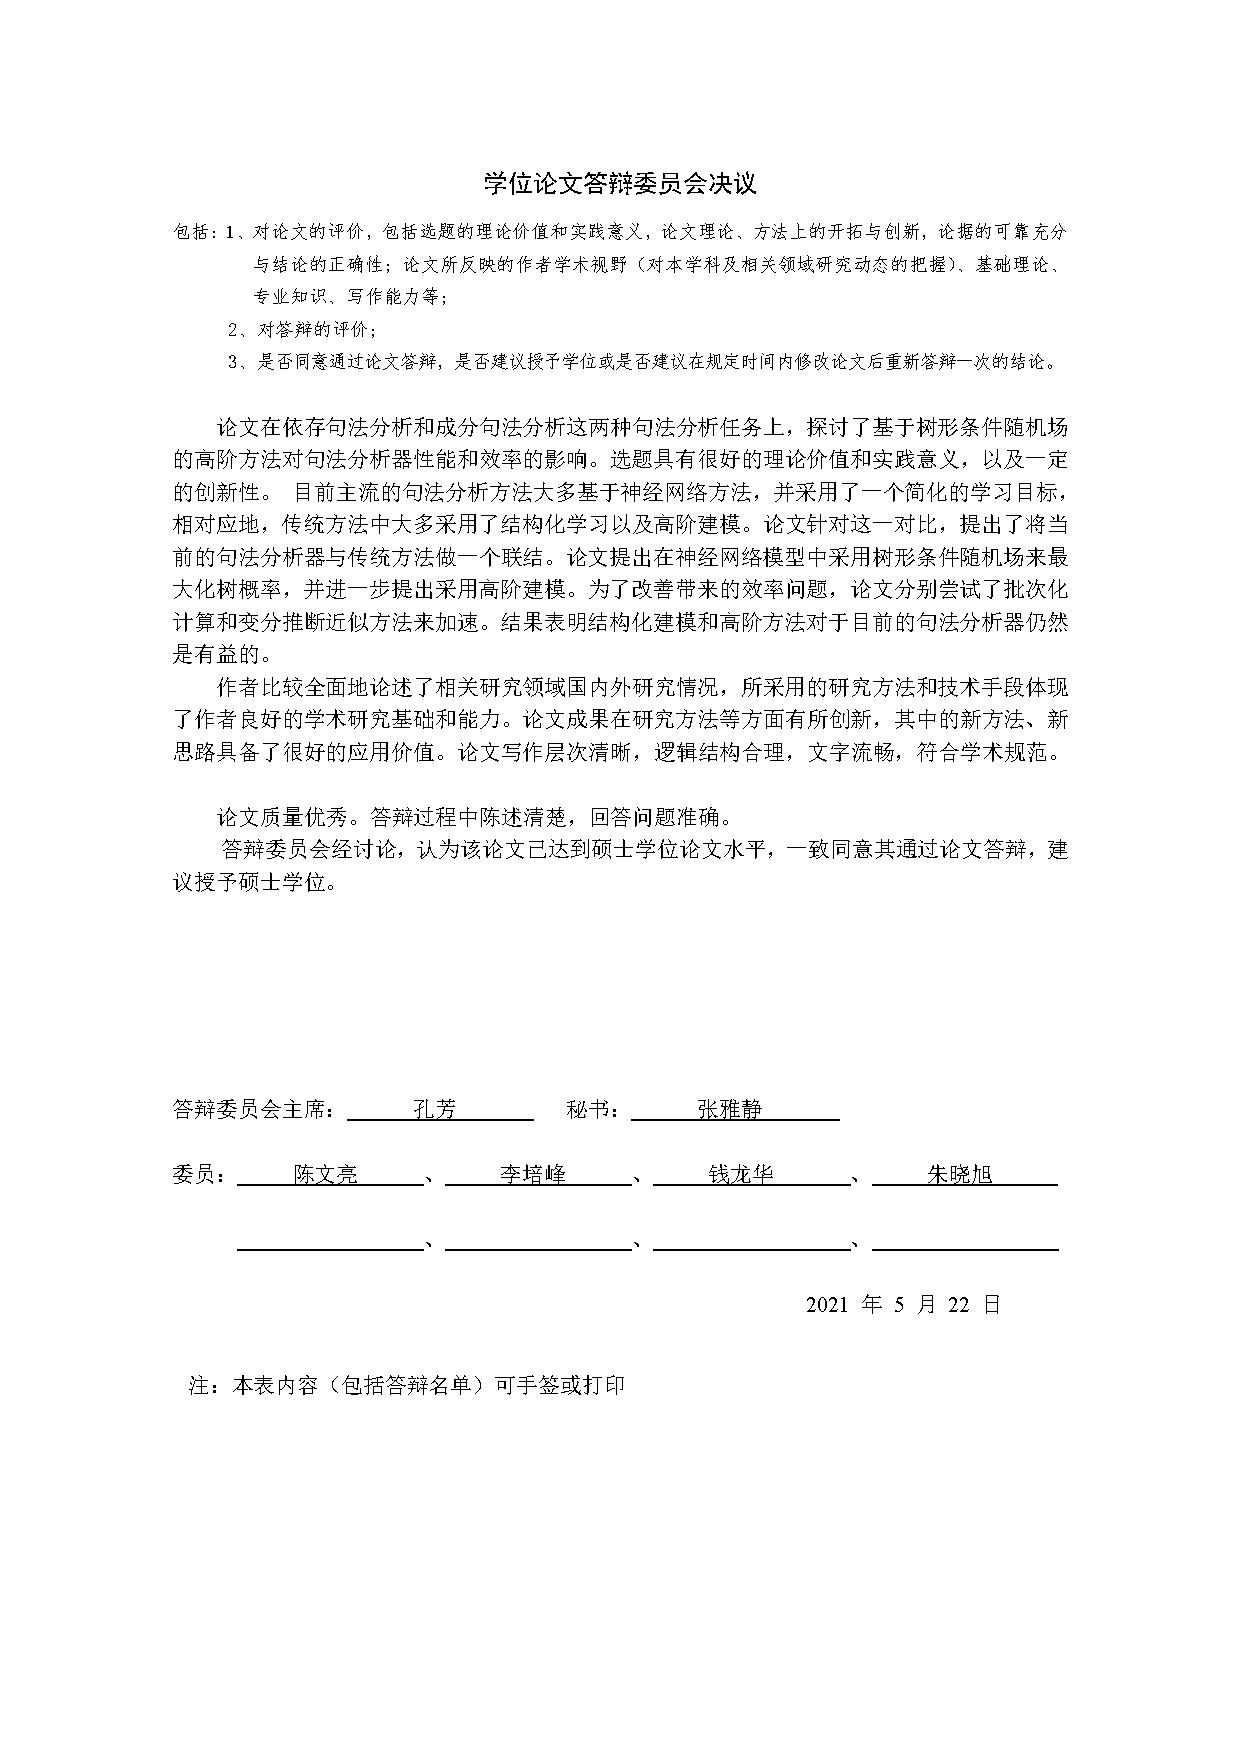
\includepdf[page=-]{pdf-pages/委员会决议.pdf}

\end{document}
